\documentclass[x11names]{beamer}
\usepackage{etex,beamerfoils}
\usepackage{array,pifont,amsmath,latexsym,epsfig,amsfonts,yfonts}
\usepackage{amstext,amsopn,amsxtra,amsgen,amsbsy,amscd,amssymb,dcolumn,graphicx,setspace,pgfplots,booktabs,natbib}
\usepackage[normalem]{ulem}
\usepackage[all]{xy}
\beamertemplatetheoremsnumbered
\setbeamertemplate{caption}[numbered]
\usetheme{Copenhagen}
\definecolor{NewBlue}{RGB}{4, 114, 155}
\definecolor{magenta}{cmyk}{0,1,0,0}
\usecolortheme[named=NewBlue]{structure}
%\usecolortheme[named=SkyBlue4]{structure}


\newcommand{\D}{\displaystyle}
\newcommand{\E}{\begin{eqnarray*}}
\newcommand{\F}{\end{eqnarray*}}
\newcommand{\EE}{\begin{eqnarray}}
\newcommand{\FF}{\end{eqnarray}}
\newcommand{\IZ}{\begin{itemize}}
\newcommand{\ZI}{\end{itemize}}
\newcommand{\EN}{\begin{enumerate}}
\newcommand{\NE}{\end{enumerate}}
\newcommand{\itemc}{\item[$\circ$]}
\newcommand{\IZdash}{\begin{itemize} \renewcommand{\labelitemi}{-}}
\newcommand{\tn}{\textnormal}

% New commands to assist Beamer
\newcommand{\itemi}{\item<1->}
\newcommand{\itemii}{\item<2->}
\newcommand{\itemiii}{\item<3->}
\newcommand{\itemiv}{\item<4->}
\newcommand{\itemv}{\item<5->}
\newcommand{\itemvi}{\item<6->}
\newcommand{\itemvii}{\item<7->}
\newcommand{\itemviii}{\item<8->}
\newcommand{\itemix}{\item<9->}
\newcommand{\itemx}{\item<10->}

\newcommand{\itemci}{\item[$\circ$]<1->}
\newcommand{\itemcii}{\item[$\circ$]<2->}
\newcommand{\itemciii}{\item[$\circ$]<3->}
\newcommand{\itemciv}{\item[$\circ$]<4->}
\newcommand{\itemcv}{\item[$\circ$]<5->}
\newcommand{\itemcvi}{\item[$\circ$]<6->}
\newcommand{\itemcvii}{\item[$\circ$]<7->}
\newcommand{\itemcviii}{\item[$\circ$]<8->}
\newcommand{\itemcix}{\item[$\circ$]<9->}
\newcommand{\itemcx}{\item[$\circ$]<10->}


\newcommand{\fr}{\frame}
\newcommand{\ft}{\frametitle}
\newcommand{\ons}{\onslide}
\newcommand{\tc}{\textcolor}

\pgfplotsset{height =7cm,compat=1.7,width=7cm,
    standard/.style={
    	unit vector ratio*=1 1 1,
        axis x line=middle,
        axis y line=middle,
        enlarge x limits=0.15,
        enlarge y limits=0.15,
        every axis x label/.style={at={(current axis.right of origin)},anchor=north west},
        every axis y label/.style={at={(current axis.above origin)},anchor=north east}
    }
}
\newcommand{\drawge}{-- (rel axis cs:1,0) -- (rel axis cs:1,1) -- (rel axis cs:0,1) \closedcycle}
\newcommand{\drawle}{-- (rel axis cs:1,1) -- (rel axis cs:1,0) -- (rel axis cs:0,0) \closedcycle}

\usetikzlibrary{patterns}
\usetikzlibrary{arrows}
\usetikzlibrary{shapes}

\renewcommand{\bibsection}{}

% Watermark example: https://texblog.org/2012/02/17/watermarks-draft-review-approved-confidential/
\usepackage{draftwatermark}
\SetWatermarkText{This content is protected and may not be shared uploaded or distributed.}
\SetWatermarkScale{0.25}
\SetWatermarkAngle{0}
\SetWatermarkColor[gray]{1.0}
\setbeamercolor{background canvas}{bg=}%transparent canvas

\title[Introduction\hspace{2em}\insertframenumber/
\inserttotalframenumber]{Introduction}
\author[Brian C. Jenkins - Computational Macroeconomics ]{Brian C.~Jenkins \\ ~ \\Econ 126: Computational Macroeconomics\\ ~ \\University of California, Irvine}

\begin{document}

\frame{\maketitle}


\fr{
\ft{Why Computational Methods for Macroeconomics}

\IZ
\item Computational tools are indispensable for many areas of economic research and particularly for macroeconomics.

\

\item Macroeconomists use computational tools to:
	\EN
	\item Solve and simulate complex dynamic models (often impossible with paper and pencil)
	\item Manage and analyze data
	\NE

\
 
\item Undergraduate economic curriculum often shields students from this knowledge for a variety of reasons (e.g., pedagogical philosophy, perceived lack of math proficiency of students, cost to faculty of course design)
\ZI

}



\fr{
\ft{Why Computational Methods for Macroeconomics}
\begin{exampleblock}{Example: RBC Model}

\IZ
\item A three-equation real business cycle (RBC) model:\pause
	\begin{align}
	C_t^{-1} & = \beta E_t\left[C_{t+1}^{-1}\left(\alpha A_{t+1} K_{t+1}^{\alpha-1}+1-\delta\right)\right] \label{eqn:euler} \\
	C_t + K_{t+1} & = A_{t}K_t^{\alpha} + (1-\delta)K_t\\
	\log A_{t+1} & = \rho \log A_t + \epsilon_{t+1}
	\end{align}
	
\itemiii Equation (\ref{eqn:euler}) implies that $C_t$ depends on the \emph{expectation} of $C_{t+1}$.

\

\itemiv But Equation (\ref{eqn:euler}) also implies that the \emph{expectation} of  $C_{t+1}$ depends on the  \emph{expectation} of $C_{t+2}$ and so on.

\ZI
\end{exampleblock}
}



\fr{
\ft{Why Computational Methods for Macroeconomics}
\begin{exampleblock}{Example: RBC Model}

\IZ
\item So computing $C_t$ requires also computing the expected path of $C_{t+1}, C_{t+2}, C_{t+3}, \ldots $ given $A_t$ and $K_t$.

\

\itemii Solving the problem \emph{analytically} (i.e., exactly with paper and pencil) would take pages of calculations and is error prone.

\

\itemiii Programmed properly, a computer can solve the problem \emph{numerically} (i.e., approximately) in less than a second.




\ZI
\end{exampleblock}
}


\fr{
\begin{figure}[h] \caption{\label{fig2} \textbf{Simulated RBC model.}}
\hspace*{-.5cm}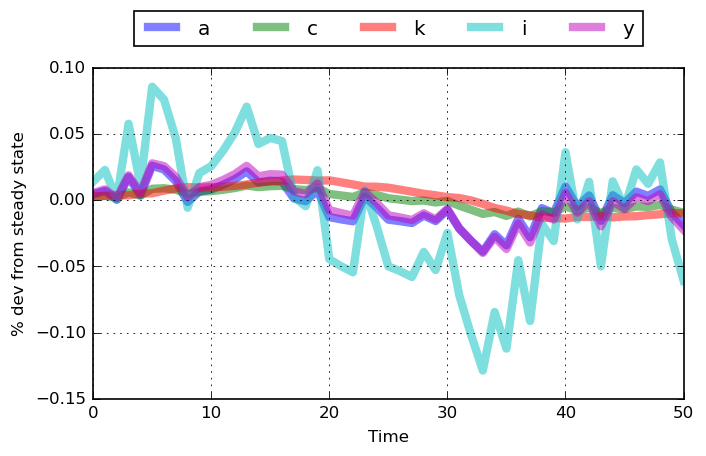
\includegraphics[height = 5cm]{fig_001_rbc_simulation.png}
\end{figure}
}



\fr{
\ft{Why Python}

\IZ
\item Macroeconomists have a lot of options:
	\EN
	\item Lower level, compiled languages: Fortran, C/C++
	\item Higher level, scripting languages: Python, Matlab, Octave, Julia, R, Stata
	\NE
	
\

\itemii The compiled languages execute more quickly, but the time investment to write code is greater.
\ZI


}


\fr{
\ft{Why Python}

\IZ
\itemi Among the scripting languages, Python has a lot of advantages:

\

	\EN
	\itemii Free and open source
	\itemiii Broad and active user base
	\itemiv Many high quality libraries for numerical and statistical computing
	\itemv Versatile: Numerical applications, web scraping, email management, web development
	\NE
	
\

\itemvi Versatility means that even if you don't become a researching macroeconomist or a financial engineer, you can still use Python.
\ZI


}


\fr{
\ft{Why Python}

\IZ
\itemi I use regularly use Python for purposes other than research:

	\IZ
	\itemi Updating graphs in lecture slides automatically
	\itemii Making animated videos for teaching purposes (e.g., \href{https://youtu.be/SdAuHSKtpmk}{https://youtu.be/SdAuHSKtpmk})
	\itemiii Sending personalized emails to students
	\itemiv Completing the DMCA takedown request form on Course Hero website
	\itemv Designing a mural for a wall in my house.
	\ZI
	
	 
\ZI
}


\fr{
\begin{figure}[h] \caption{\label{fig2} \textbf{Mural: Design concept.} Colors are taken from the Sherwin Williams color catalog.}
\hspace*{-.5cm}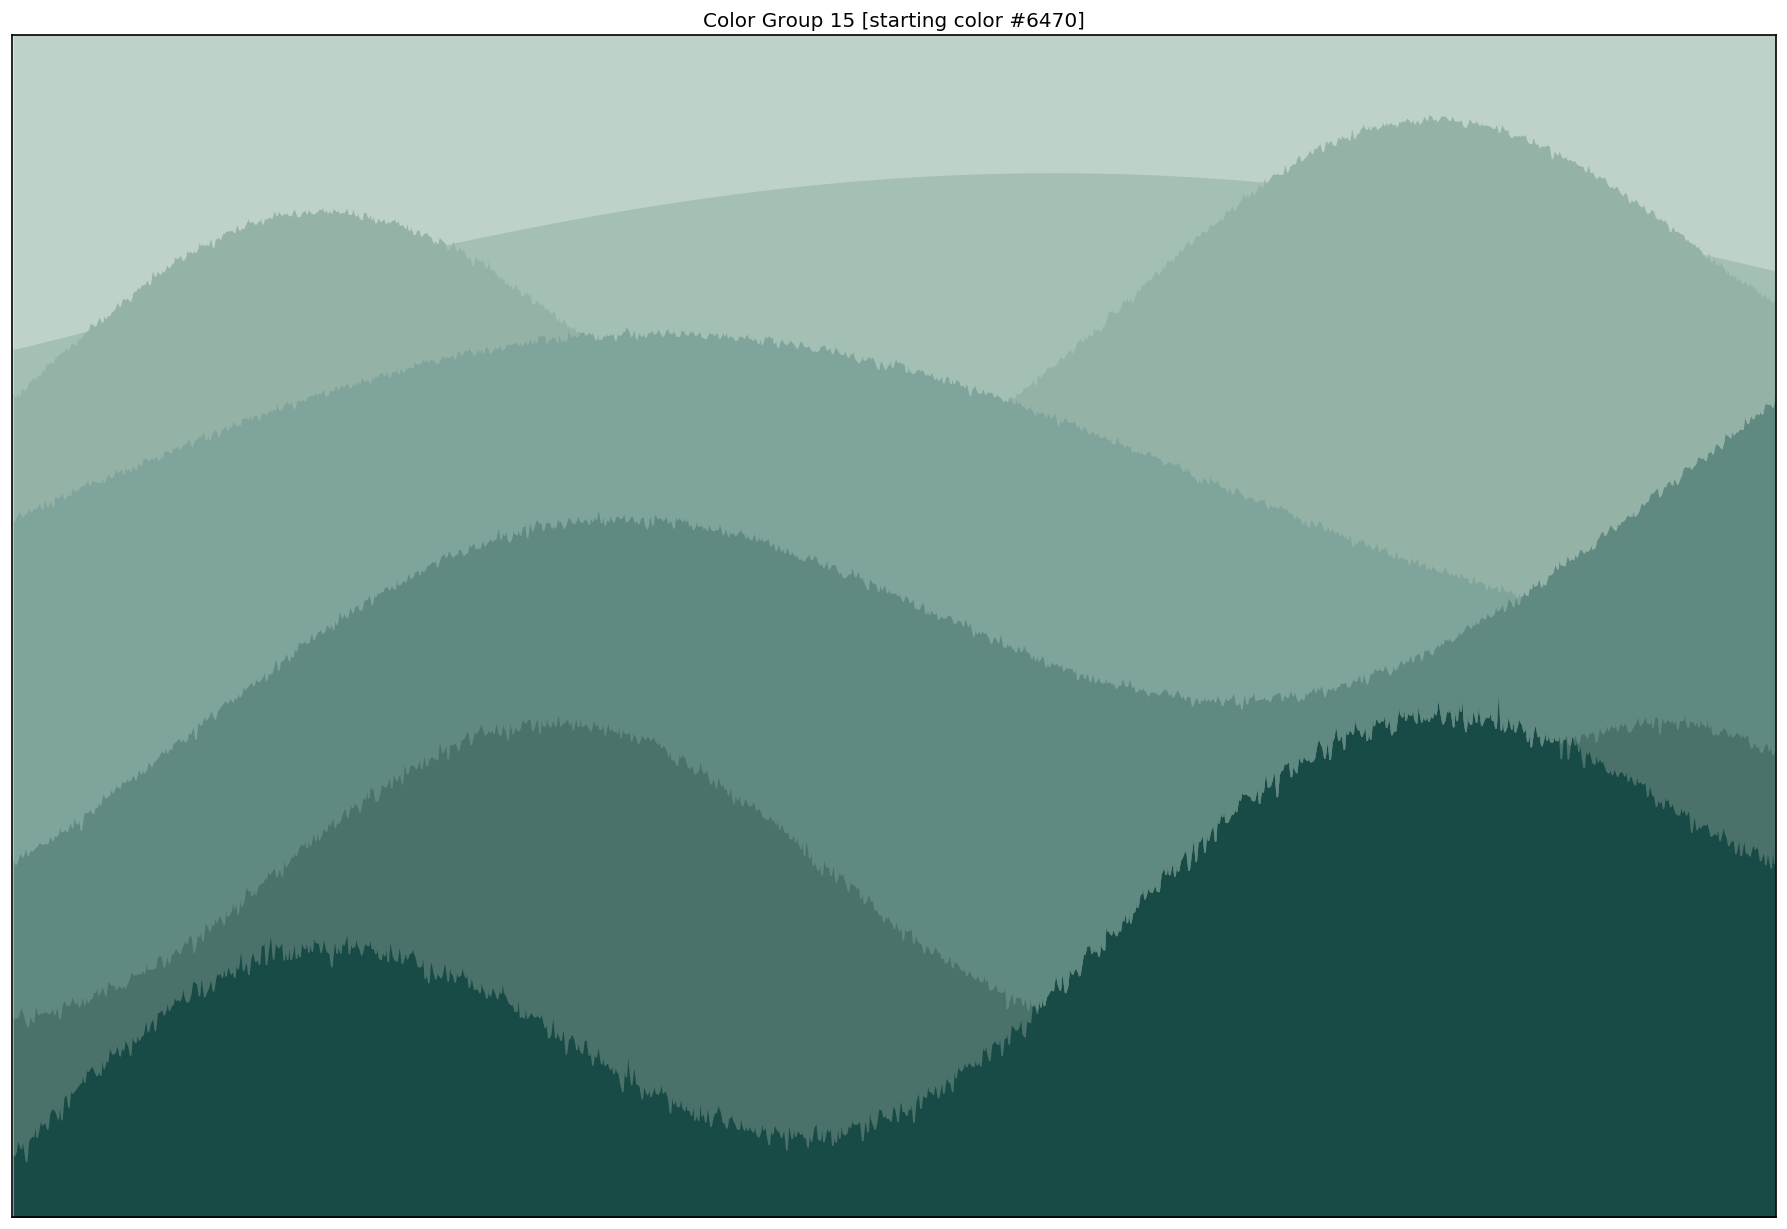
\includegraphics[height = 5cm]{fig_001_mural_concept.png}
\end{figure}
}

\fr{
\begin{figure}[h] \caption{\label{fig2} \textbf{Mural: key coordinates.}}
\hspace*{-.5cm}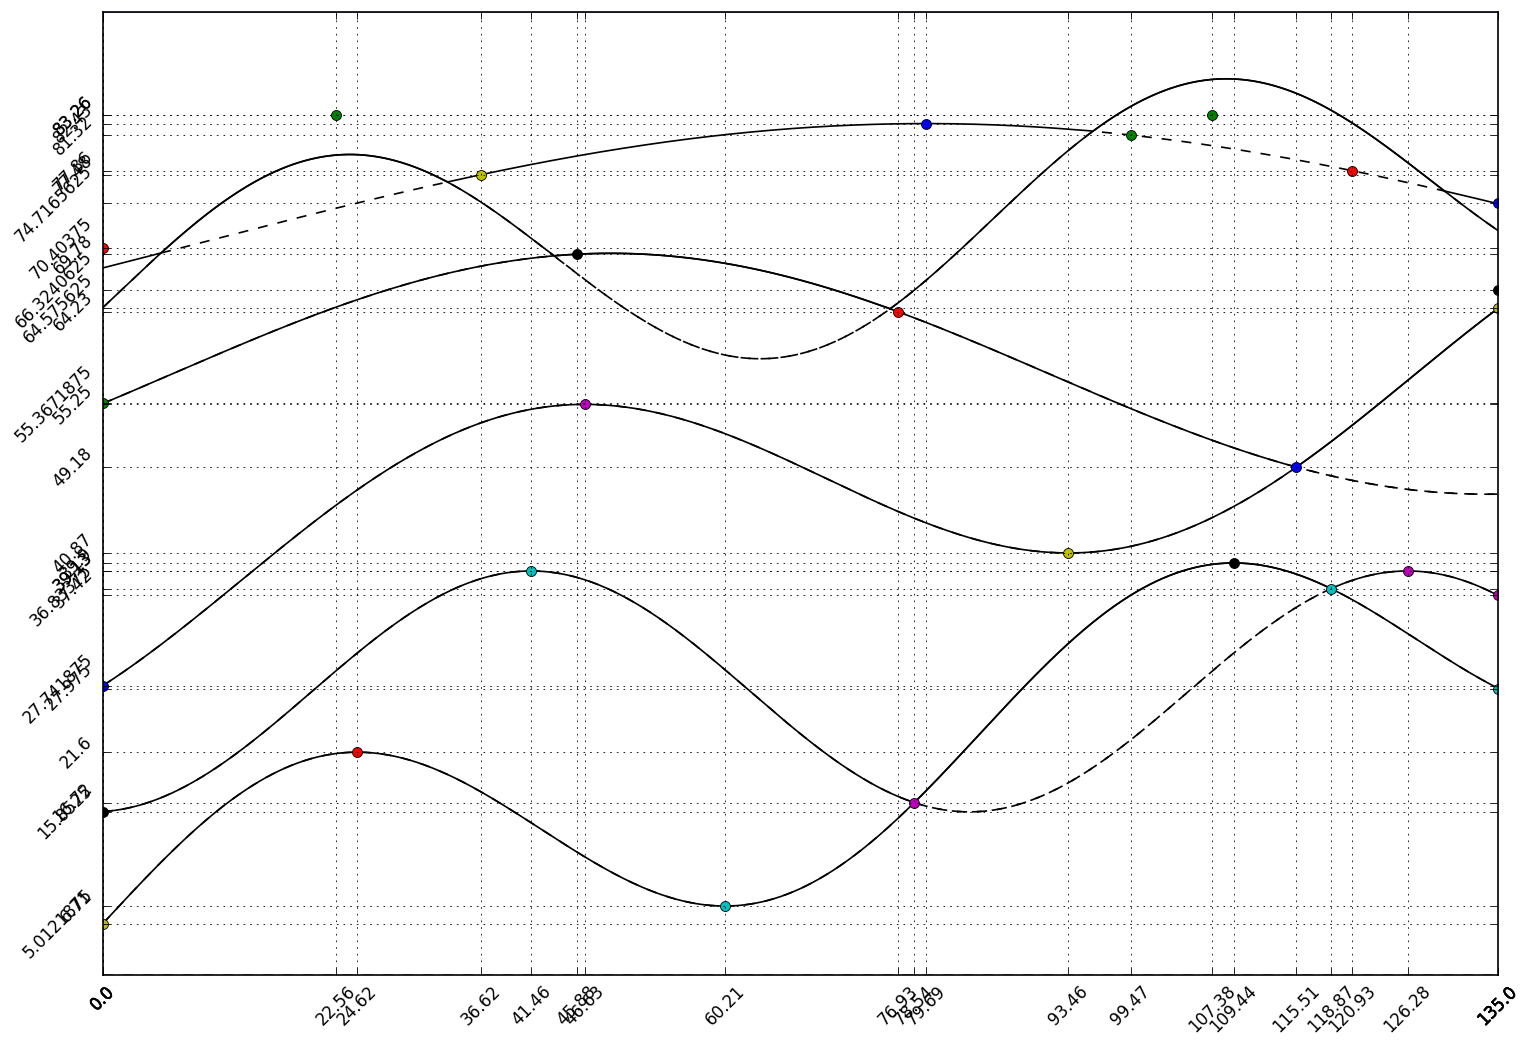
\includegraphics[height = 5cm]{fig_001_mural_interior_boundary_points.png}
\end{figure}
}

\fr{
\begin{figure}[h] \caption{\label{fig2} \textbf{Mural: final result.}}
\hspace*{-.5cm}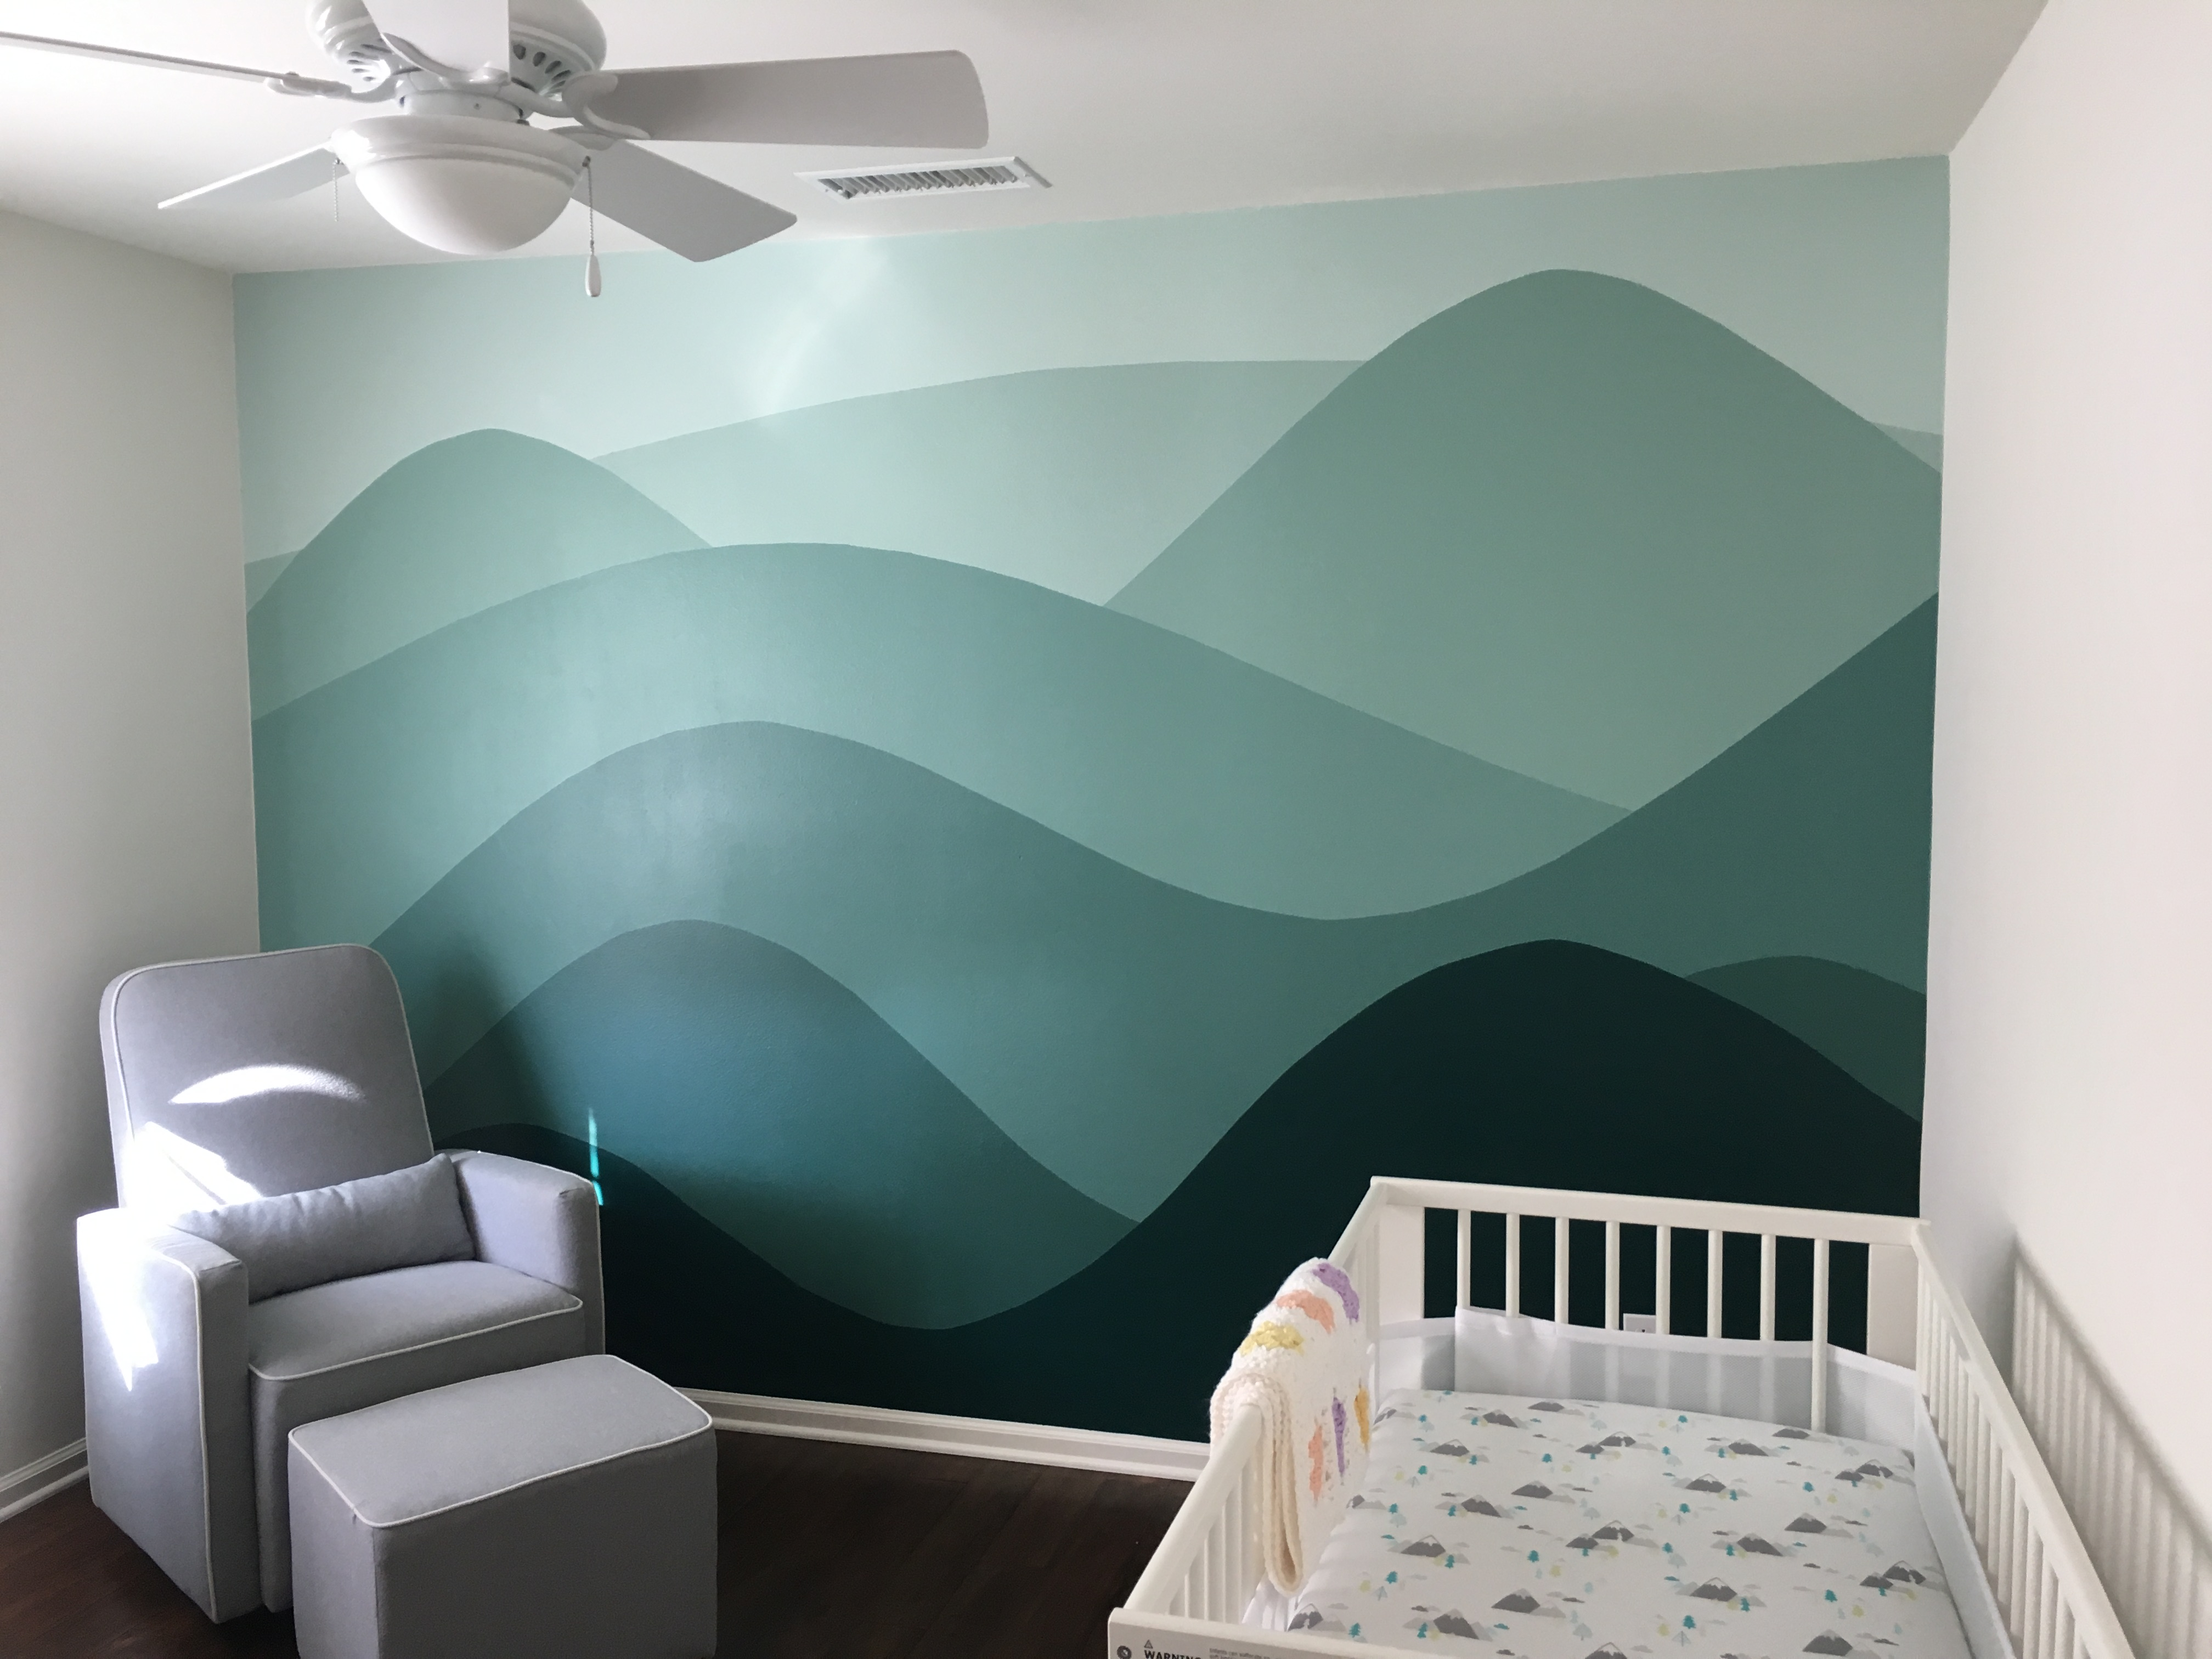
\includegraphics[height = 5cm]{fig_001_mural_finished.jpg}
\end{figure}
}




\fr{
\ft{Overview of the Course}

\IZ
\item In this course you will learn:

	\IZ
	\itemii Basic Python programming skills
	\itemiii How to use Python to manage data and do basic statistics including linear regression
	\itemiv How to use Python to simulate linear dynamic models.
	\itemv How to approximate nonlinear dynamic stochastic models.
	\itemvi The basics of the real business cycle (RBC) and  new Keynesian modeling approaches
	\itemvii Critiques and criticisms of both business cycle modeling approaches
	\ZI
\ZI

}


\fr{
\ft{Overview of the Course}

\IZ
\item The course presumes no programming experience

\

\item My philosophy is that coding is like cooking: it's often sufficient to learn just what you need to know in order to make what you're trying to make
\ZI

}




\end{document}